\begin{activity} \label{A:5.6.2}  A car traveling along a straight road is braking and its velocity is measured at several different points in time, as given in the following table.  Assume that $v$ is continuous, always decreasing, and always decreasing at a decreasing rate, as is suggested by the data.
\begin{center}
\begin{tabular}{|l|c|c|c|c|c|c|c|}
\hline
seconds, $t$ & 0 & 0.3 & 0.6 & 0.9 & 1.2 & 1.5 & 1.8 \\
\hline
Velocity in ft/sec, $v(t)$ & 100 & 99 & 96 & 90 & 80 & 50 & 0 \\
\hline
\end{tabular}
\end{center}
\ba
	\item Plot the given data on the set of axes provided in Figure~\ref{F:5.6.Act2} with time on the horizontal axis and the velocity on the vertical axis.
	\item What definite integral will give you the exact distance the car traveled on $[0,1.8]$?
	\item Estimate the total distance traveled on $[0,1.8]$ by computing $L_3$, $R_3$, and $T_3$.  Which of these under-estimates the true distance traveled?
	\item Estimate the total distance traveled on $[0,1.8]$ by computing $M_3$.  Is this an over- or under-estimate?  Why?
	\item Using your results from (c) and (d), improve your estimate further by using Simpson's Rule.
	\item What is your best estimate of the average velocity of the car on $[0,1.8]$?  Why?  What are the units on this quantity?
\ea
\begin{figure}[h]
\begin{center}
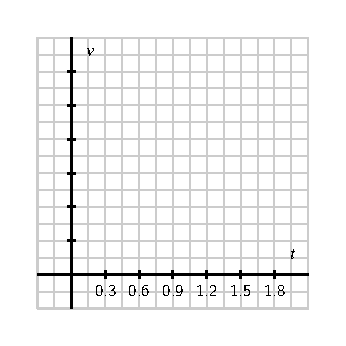
\includegraphics{figures/5_6_Act2.eps}
\caption{Axes for plotting the data in Activity~\ref{A:5.6.2}.} 
\label{F:5.6.Act2}
\end{center}
\end{figure}
\end{activity}
\begin{smallhint}
\ba
	\item Small hints for each of the prompts above.
\ea
\end{smallhint}
\begin{bighint}
\ba
	\item Big hints for each of the prompts above.
\ea
\end{bighint}
\begin{activitySolution}
\ba
	\item Solutions for each of the prompts above.
\ea
\end{activitySolution}
\aftera